\chapter{Agents}
Artificial intelligence, or AI, is the field that studies the synthesis and analysis of computational agents
that act intelligently.\newline
An agent is something that acts in an environment/it does something and we are interested in what an agent does,
that is, how it acts, so we judge an agent by its actions.

An agent acts \emph{intelligently} when what it does is appropriate given the circumstances and its goals,
it is flexible to changing environments and changing goals, it learns from experience and 
it makes appropriate choices given its perceptual and computational limitations.

\begin{defi}
A \emph{computational agent} is an agent whose decisions about its actions can be explained 
in terms of computation.
\end{defi}
We have that the central scientific goal of AI is to understand the principles that make intelligent behavior
possible in natural or artificial systems, instead the central engineering goal of AI is the design and synthesis of
useful, intelligent artefacts, agents, that are useful in many applications.\newline
This is done by the analysis of natural and artificial agents, formulating and testing hypotheses about
what it takes to construct intelligent agents and in the end designing, building, and experimenting
with computational systems that perform tasks commonly viewed as requiring intelligence.

Artificial Intelligence is not the opposite of real Intelligence, infact intelligence cannot be fake, so
if an artificial agent behaves intelligently, it is intelligent and it is only the external behavior
that defines intelligence (weak AI).

Artificial intelligence is real intelligence created artificially and we can use different test to 
estabilish if AI is intelligent: \emph{Turing test} where only external behavior counts and \emph{Winograd schemas}
as a test of intelligence, where we asks "The city councilmen refused the demonstrators a permit 
because they feared violence. Who feared violence?" and "The city councilmen refused the demonstrators a permit
because they advocated violence. Who advocated violence?".\newline
These questions are difficult for a machine because it has not the knowledge of context.

The obvious naturally intelligent agent is the human being and the human intelligence
comes from three main sources:
\begin{enumerate}
    \item biology: Humans have evolved into adaptable animals that can survive in various habitats.
    \item culture: Culture provides not only language, but also useful tools, useful concepts, and 
          the wisdom that is passed from parents and teachers to children.\newline
          Language, which is part of culture, provides distinctions in the world that should be noticed for learning.
    \item life-long learning (experience): Humans learn throughout their life and accumulate knowledge and skills.
\end{enumerate}
Another form of intelligence is \emph{social intelligence}, the one exhibited by communities and organizations.

Three aspects of computation that must be distinguished:
\begin{enumerate}
    \item Design time computation, that goes into the design of the agent
    \item Offline computation, that the agent can do before acting in the world
    \item Online computation, the computation that is done by the agent as it is acting.
\end{enumerate}
Designing an intelligent agent that can adapt to complex environments and changing goals is a major challenge, so 
to reach this ultimate goal, two strategies are possible:
\begin{enumerate}
    \item simplify environments and build complex reasoning systems for these simple environments.
    \item build simple agents for natural/complex environments, simplifying the tasks.
\end{enumerate}
The design process of an agents has the following phases, that can be viewed on figure \ref{img:designProcess}:
\begin{enumerate}
    \item Define the task: specify what needs to be computed
    \item Define what constitutes a \emph{solution} and its quality: optimal solution,
          satisficing solution, approximately optimal solution, probable solution.
    \item Choose a formal representation for the task; this means choosing how to represent knowledge for the task
          and this includes representations suitable for learning.
    \item Compute an output
    \item Interpret output as a solution
\end{enumerate}

\begin{figure}
    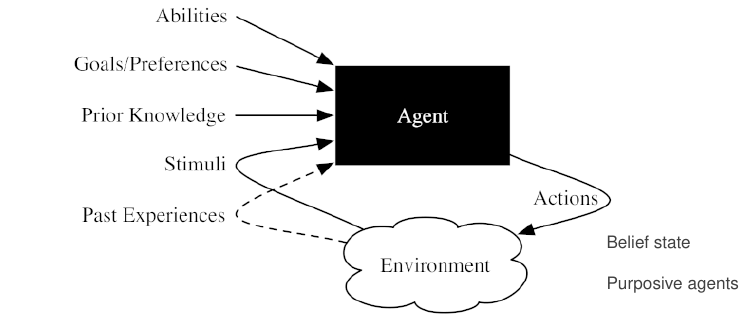
\includegraphics[width=0.8\textwidth]{Images/agents}
    \caption{Design Process of AI agents}
    \label{img:designProcess}
\end{figure}
A model of the world is a symbolic representation of the beliefs of the agents about the world, 
so it is necessarily an abstraction.\newline
More abstract representations are simpler and human-understandable, but they
may be not effective enough and low level descriptions are more detailed and accurate but introduce complexity.

Multiple level of abstractions are possible (hierarchical design), but usually two levels are considered:
\begin{enumerate}
    \item The \emph{knowledge level}: what the agent knows and its goals
    \item The \emph{symbol level}: the internal representation and reasoning algorithms
\end{enumerate}

In agent design we consider these aspects, with a summary foundable in figure \ref{img:summary}:
\begin{description}
    \item [Modularity: ] is the extent to which a system can be decomposed into interacting modules
                         and it is a key factor for reducing complexity.\newline
                         In the modularity dimension, an agent’s structure is one of the following:
                         \begin{itemize}
                            \item \emph{flat} where there is no organizational structure.
                            \item \emph{modular}, which the system is decomposed into interacting modules
                                  that can be understood on their own.
                            \item \emph{hierarchical}, which the system is modular, and the modules themselves are
                                  decomposed into simpler modules and the agent reasons at 
                                  multiple levels of abstraction.
                        \end{itemize}

    \item [Planning Horizon: ] is how far ahead in time the agent plans and in this dimension an agent
                               is one of the following:
                               \begin{itemize}
                                    \item \emph{Non-planning agent}, that does not look at the future.
                                    \item \emph{Finite horizon} planner, where agent looks for a fixed finite
                                          number of stages and it is greedy if only looks one time step ahead.
                                    \item \emph{Indefinite horizon} planner is an agent that looks ahead some finite,
                                          but not predetermined, number of stages.
                                    \item \emph{Infinite horizon} planner is an agent that keeps planning forever
                               \end{itemize}
    \item [Representation: ] concerns on how the state of the world is described and a state of the world
                             specifies the agent’s internal state (its belief state) and the environment state.\newline
                             We have $3$ type of representation, from simple to complex:
                             \begin{itemize}
                                \item \emph{atomic} states, as in problem solving.
                                \item \emph{feature-based} representation: set of propositions that are true or
                                      false of the state, properties with a set of possible values. 
                                \item Individuals and relations (often called relational representations) and 
                                      is the Representations at the expressive level of FOL (or contractions).
                             \end{itemize}

    \item [Computational limit: ] an agent must decide on its best action within time constraints or other
                                  constraints in computational resources (memory, precision, \dots).\newline
                                  The computational limits dimension determines whether an agent has
                                  \emph{perfect rationality}, where an agent is able to reasons about the best action
                                  without constraints and \emph{bounded rationality}, where an agent decides
                                  on the best action that it can find given its computational limitations.\newline
                                  An \emph{anytime algorithm} is an algorithm where the solution quality improves
                                  with time and to take into account bounded rationality, an agent must decide
                                  whether it should act or reason for longer.

    \item [Learning: ] is necessary when the designer does not have a good model and the learning dimension 
                       determines whether knowledge is given in advance or knowledge is learned from data or 
                       past experience.\newline
                       Learning typically means finding the best model that fits the data and
                       produces a good predictive model and in this course only modelling formalisms
                       and approaches are dealt, infact all the issues concerned with learning
                       are dealt in the Machine Learning course.

    \item [Uncertainty: ] is divided into two dimensions:
                          \begin{enumerate}
                            \item uncertainty from sensing/perception (fully observable, partially observable states).
                            \item uncertainty about the effects of actions (deterministic, stochastic) and 
                            when the effect is stochastic, there is only a probability distribution
                            over the resulting states.
                          \end{enumerate}
    \item [Preference: ] considers whether the agent has goals or richer preferences:
                         \begin{itemize}
                            \item A \emph{goal} is either an achievement goal, which is a proposition to be true
                                  in some final state, or a maintenance goal, a proposition that 
                                  must be true in all visited states.
                            \item \emph{Complex preferences} involve trade-offs among the desirability of
                                  various outcomes, perhaps at different times.\newline
                                  An \emph{ordinal preference} is where only the ordering of the preferences is
                                  important, instead a \emph{cardinal preference} is where the 
                                  magnitude of the values matters and States are evaluated by utility functions.
                         \end{itemize}

    \item [Number of Agents: ] considers whether the agent explicitly considers other agents:
                               \begin{itemize}
                                    \item \emph{Single agent} reasoning means the agent assumes that there are no
                                          other agents in the environment or that all other agents are 
                                          “part of nature”, and so are non-purposive.
                                    \item \emph{Multiple agent} reasoning means the agent
                                          takes the reasoning of other agents into account and this occurs when
                                          there are other intelligent agents whose goals or preferences depend,
                                          in part, on what the agent does or if the agent must communicate
                                          with other agents.
                               \end{itemize}

    \item [Interaction: ] considers whether the agent does:
                          \begin{itemize}
                            \item \emph{offline reasoning}, where the agent determines what to do before
                                  interacting with the environment.
                            \item \emph{online reasoning}, where the agent must determine what action to do 
                                  while interacting in the environment, and needs to make timely decisions.
                          \end{itemize}
                          More sophisticated agents reason while acting and this includes long-range
                          strategic reasoning as well as reasoning for reacting in a timely manner to
                          the environment.
\end{description}

\begin{figure}
    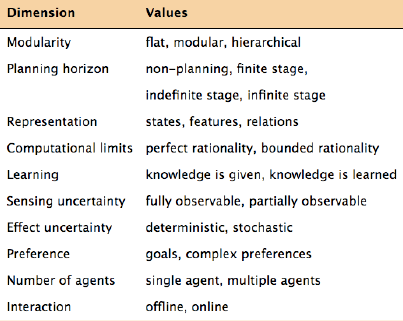
\includegraphics[width=0.8\textwidth]{Images/summary}
    \caption{Summary of Agent Design consideration}
    \label{img:summary}
\end{figure}

\begin{defi}
An agent is something that interacts with an environment, receiving information through its sensors and
acts in the world through actuators (effectors).\newline
A robot is an artificial purposive embodied agent and also a computer program is a software agent
\end{defi}
An agent is made up of a body and a controller, where the controller receives percepts from the body and
sends commands to the body.\newline
A body includes sensors that convert stimuli into percepts and actuators that convert commands into actions.
Both sensor and actuators can be uncertain, the controller is the brain of an agent and in the end
an agent system includes an agent and the environment in which it acts.\newline
In figure \ref{img:agentSystem} is possible to see the structure of an generic agent system.

\begin{figure}
    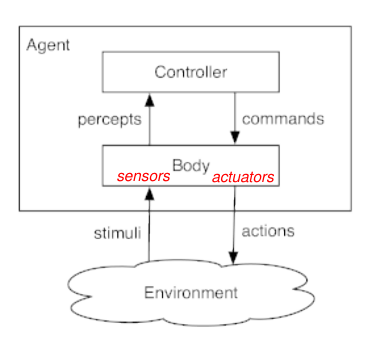
\includegraphics[width=0.6\textwidth]{Images/agent}
    \caption{Structure of an generic agent system}
    \label{img:agentSystem}
\end{figure}

Agents act in time, we have $T$ that is the set of time points, and we assume that $T$ has a start $(0)$
totally ordered, discrete, and each $t$ has a next time $t + 1$.\newline
We have an agent history that at time $t$ has percepts up to $t$ and commands up to $t - 1$ and we 
have also \emph{causal transduction} (usually implements by a controller), a function from history to commands,
called causal because only previous and current percepts and previous commands can be considered.

However, complete history is usually not available and we have only the memory of it:
the memory or belief state of an agent at time $t$ is all the information the agent
has remembered from the previous times and the behavior of an agent is described by two functions:
\begin{itemize}
    \item A \emph{belief state} transition function $S \times P \to S$, where $S$ is the set of belief states 
          and $P$ is the set of percepts.
    \item A \emph{command} function $S \times P \to C$, where $C$ is the set of commands.
\end{itemize}
The controller implements a command function (an approximation of a causal transduction) and 
with a single controller it is difficult to reconcile the slow reasoning about complex high-level goals
with the fast reaction that an agent needs for lower-level tasks such as avoiding obstacles.\newline
In figure \ref{img:agentFunctions} is possible to note the agent functions that should be implemented 
at each layer of our agent.

\begin{figure}
    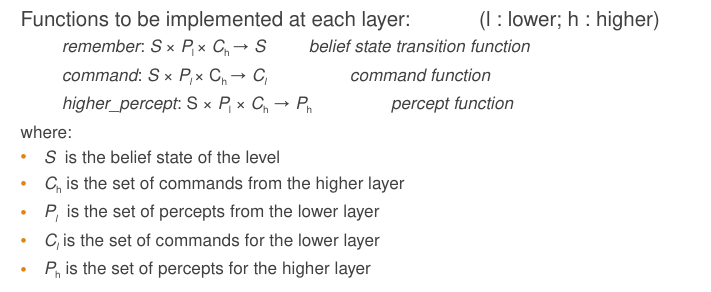
\includegraphics[width=0.8\textwidth]{Images/agentFunctions}
    \caption{Agent Functions to implement at each layer}
    \label{img:agentFunctions}
\end{figure}
high-level reasoning, is often discrete and qualitative
• low-level reasoning is often continuous and quantitative
A controller that reasons in terms of both discrete and continuous values
is called a hybrid system.

The notion of belief state is quite general, most agents need to keep a model of the word and update it while acting
and there are $2$ extremes:
\begin{enumerate}
    \item the agent possess a very good predictive model, so it does not need to use perceptions to update the model
    \item purely reactive systems do not have a model, and decide only on the basis of perceptions
\end{enumerate}
In the general case the agent uses a combination of prediction and sensing:
\begin{itemize}
    \item In Bayesian reasoning (under uncertain information) the estimation
          of the next belief state is called \emph{filtering}.
    \item In alternative, more complex models of the world can be kept and updated, for
          example through vision and image processing.
\end{itemize}
Knowledge of a specific domain may also be represented explicitly and used to decide the action and 
the \emph{knowledge base} contains general rules and specific/contingent facts in declarative form.\newline
The KB is built offline, built by designers or learned from data and a domain ontology gives meaning
to symbols used to represent knowledge; knowledge may be then updated and used to decide actions during
operation.






